\chapter{Sprint 4}
\label{chap:S5}

In the fourth sprint, the 8th and 9th week of the project, the system design is finalized. It was the period when the whoe group was working confidently with implementation and report writing. We had already started modifying the system in the previous sprint, and the whole group knew what tasks they had been assigned. The goal of the sprint was to complete the system with all modifications we had decided upon during the previous sprint, and completing as much of the report as possible.

\section{Sprint plan}
\label{sec:S5Plan}

The plan was fairly clear this sprint. Tasks were given a priority and a time estimate. Tasks with a priority of Major had to be completed as soon as possible, then tasks with Normal priority, and finally Low priority tasks if time permitted. Event registration was the system this sprint would focus the most on, as well as a redesign of the front page based on the suggestions given at the presentation in Oslo during sprint 3.

\paragraph{} As part of the plan for a new design, we would start looking into the Google design guidelines for web pages, especially looking for tips on color changes. Other plans included implementing sharing to other social media, designing logos for each interest. We also spent some time discussing the domain name for the site, and would advise the customers in setting up the site.

\section{Duration and workload}
\label{sec:S4Duration}

\begin{minipage}{\linewidth}
\centering
\setlength{\tabcolsep}{22pt}
\textbf{Sprint 4:} 
\smallskip
\rowcolors{1}{blue!20}{blue!10}
\begin{tabular}{ |l l| }
	\hline
	\it{Duration} & 2 weeks \\
	\it{Start} & October 20th. \\
	\it{End} & November 2nd. \\
	\it{Workload} & Hours spent by the entire group on Sprint 4. \\
	\it{Goal} & 20-25 hours per person \\
	\hline
\end{tabular}
\end{minipage}\\%
%
\begin{minipage}{\linewidth}
\setlength{\tabcolsep}{15pt}
\centering
\rowcolors{1}{blue!20}{blue!10}
\begin{tabular}{ |l|l| }
	\hline
	\multicolumn{2}{|c|}{\cellcolor{gray!25} Workload} \\
	\hline
	\it{Planning} & 25 hrs\\
	\it{Development} & 58 hrs\\
	\it{Design} & 20 hrs\\
	\it{Documentation} & 83 hrs\\
	\it{Testing} & 10.5 hrs\\
	\hline
	\textbf{\textit{Total Workload}} & 196.5 hrs\\
	\hline
\end{tabular}
%Caption here
\captionof{table}{Workload of Sprint 4. \label{tab:S4Workload}} 
\end{minipage}

The group's amount of work went down compared to the previous sprint. Some people were away, and ill. It is further discussed in section \ref{sec:S5GroupDynamics}.

\section{Sprint backlog}
\label{sec:S4Backlog}

\begin{minipage}{\linewidth}
\setlength{\tabcolsep}{12pt}
\centering
\rowcolors{1}{blue!20}{blue!10}
\begin{tabular}{|p{1cm}|p{4cm}|p{2cm}|p{2cm}|}
\hline
\cellcolor{gray!25} ID & \cellcolor{gray!25} Description & \cellcolor{gray!25} Estimated Time & \cellcolor{gray!25} Actual Time \\
\hline
CDP-25 & \it{Design of home page} & 2d & 2d2h \\
CDP-13 & \it{Navigation between pages} & 4h & 4h \\
CDP-8 & \it{Event creation} & 3d & 3d4h30m \\
CDP-21 & \it{Photos should display more details (when was the photo uploaded, by whom)} & 4h & 4h \\ 
CDP-36 & \it{Photo rating} & 12 hrs & 1d \\
D4.1 & \it{Icons fo the different interests} & 3hrs & 4hrs \\
RPT-41 & \it{Finish Sprint 1 for the report} & 3hrs & 3hrs \\
RPT-42 & \it{Sprint 2} & 18h & 1d2h \\
RPT-43 & \it{Sprint 3} & 12h & 12h \\
RPT-47 & \it{Introduction} & 3h & 3h \\
RPT-71 & \it{Risk management} & 1d & 1d2h \\
RPT-72 & \it{Quality Assurance} & 5h & 5h \\
RPT-29 & \it{Restructuring/finishing preliminary studies} & 6h & 5h \\
R4.1 & \it{Proofreading} & 5h & 5h \\
\hline
\end{tabular}
\captionof{table}{Backlog for sprint 4.} 
\end{minipage}\\%
%
\begin{minipage}{\linewidth}
\setlength{\tabcolsep}{12pt}
\centering
\rowcolors{1}{blue!20}{blue!10}
\begin{tabular}{|p{1cm}|p{4cm}|p{2cm}|p{2cm}|}
\hline
\multicolumn{4}{|c|}{\cellcolor{gray!25} CDP-25} \\
\hline
CDP-31 & \it{Implement the new 2D search design} & 6h & 4h \\
CDP-32 & \it{Search by address on the map.} & 6h & 6h \\
\hline
\end{tabular}
\end{minipage}


\section{Design and implementation}
\label{sec:S4DesignImpl}

\paragraph{} This sprint we did a redesign of the photos page, which would become the new start page. We also implemented many of the features that had been asked for by the end users at the Oslo presentation. Features include the need for a larger map when searching for photos, address search, an overlay for viewing events, and changes needed before deploying the prototype to the costomer's domain.

\begin{figure}[ht!]
  \centering
  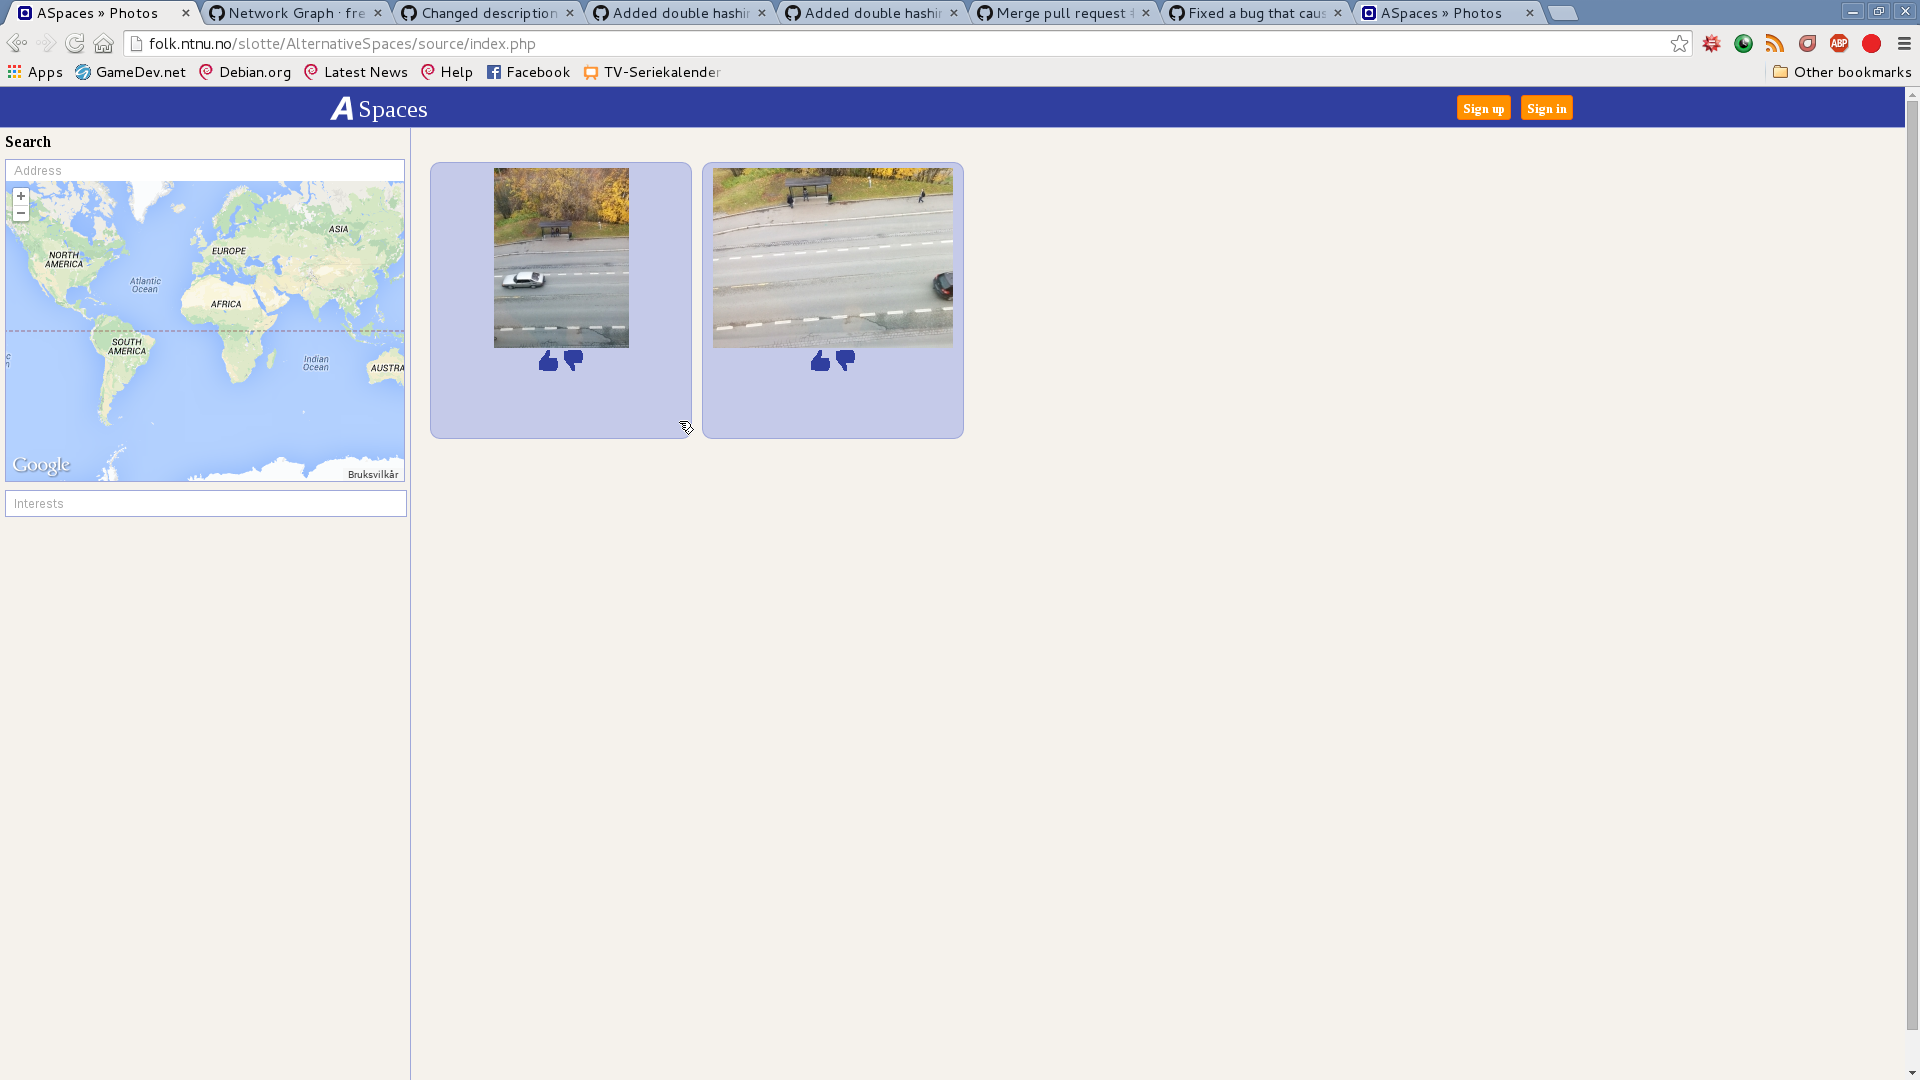
\includegraphics[width=\linewidth]{./img/webpage/27Oct/Frontpage27Oct}
  \caption{The first iteration of the new design for the front page.}
  \label{fig:S4DesignImplFront27Oct}
\end{figure}

\paragraph{} As mentioned in \ref{subsec:S2PresentationFeedback}, the most important problem with our site, after the lack of a mobile app, was the small size of the search map when in the photos view. As shown in figure \ref{fig:S4DesignImplFront27Oct}, we quadrupled the size of the map, which greatly increased the usability, and improved the use of space, especially on screens with high resolution.

\paragraph{} The next feature the youth had asked for was the ability to search for locations by address. This was added 


%TODO PARTS NOT PLACED
%We agreed upon some guidelines to follow while writing report, such as using figures, tables and pictures, to use the suggestion mode in the google docs, so that they would enhance the quality of the report and planned to document the report chapters into Latex.
%There has been a discussion about the domain name for the Website and later the customer gave the domain name as MY SPLOT, which is a combination of spot and lot, ideally suitable name for youth to hangout.